\section{Cloud Based Processing, Storage and Inference}
\label{cloud_services}
%Need to discuss Lambda which takes raw data to pp data bucket here
\subsection{Laptop to Cloud Pipeline}
\subsubsection{API Gateway}
In this section we discuss the entry way into the AWS Cloud. The API Gateway allows us to take any data produced the Edge location either from the end-user or the Edge nodes deployed and securely redirect them to storage and analysis endpoints. Figure \ref{fig:api_gateway_methods} shows how various URLs an be used to upload and send data to different buckets or endpoints. Usage of Sagemaker's endpoints are discussed later, but to get data from the edge to the cloud, the S3 endpoints are used by API Gateway. For example, doing a \textit{PUT} request to the provided URL from API Gateway, with the body of the request filled with the JSON object to be uploaded, would store the data file with the new Key value into the requested S3 bucket.

\begin{figure}[ht]
    \centering
    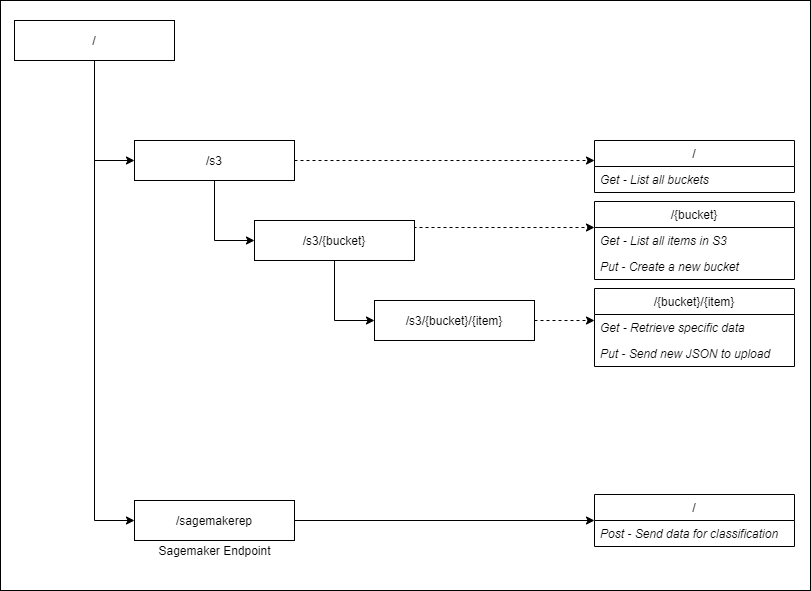
\includegraphics[width=1\linewidth]{pages/Chapter4/Chapter 4 Images/api_gateway_1.png}
    \caption{API Gateway Resources and Attached Methods}
    \label{fig:api_gateway_methods}
\end{figure}


\subsubsection{Lambda - Data Pre-processing on the Cloud}
\label{cloud_lambda}
Once the data has been prepared and the API Gateway setup, then Lambda services can be triggered to react to New Object events on S3. It can be setup such that every new object will trigger the Lambda function, however it may be the case that not all the 5 JSON files will have been uploaded as part of the Laptop to Cloud Pipeline. This would mean the pre-processing would be incomplete. One solution to this problem is for all 5 JSON files to be uploaded first and then upload a separate file with .complete file type. This was arbitrary chosen, and Lambda can be setup to trigger on only .complete files that upload to S3. This ensures that all 5 JSON files will exist before the functions searches for them. The diagram in Figure \ref{fig:s3_lambda_s3} shows this process and how it will be accomplished diagramatically.

\begin{figure}[ht]
    \centering
    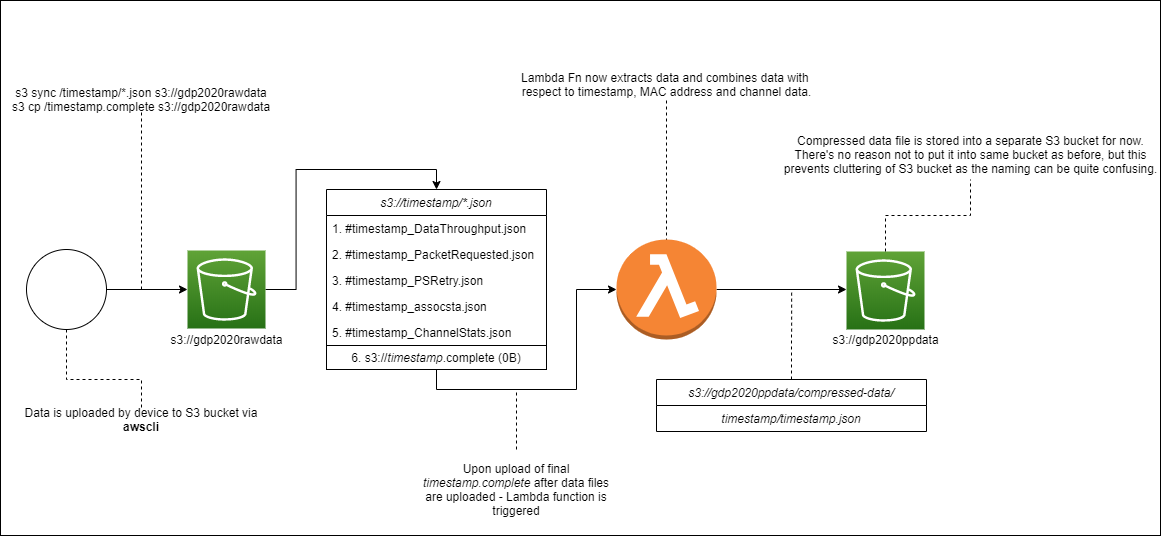
\includegraphics[width=1\linewidth]{pages/Chapter3/Chapter 3 images/S3_to_Lambda_to_S3.png}
    \caption{Triggering Lambda from S3 Uploads - \textit{The full scale diagram can be seen in Appendix E} [\ref{appendix:data_flow_from_laptop_to_cloud}]}
    \label{fig:s3_lambda_s3}
\end{figure}

\subsection{Machine Learning on the Cloud}

The following pipeline shown in \ref{appendix:ML process pipeline} summarizes the machine learning processes that will be carried out.
Firstly, the problem in building the machine learning model was identified from the telemetry data collected from the router. With careful analysis over the parameters collected, data throughput rate is chosen to create a class (target variable) labeled as data throughput strength which will be used to build the machine learning model. Data throughput rate is chosen because it is able to show the amount of data which can be received and sent within a given time span. This enables the prediction of a network performance based on the classification of data throughput strength.

\begin{figure}[ht]
    \centering
    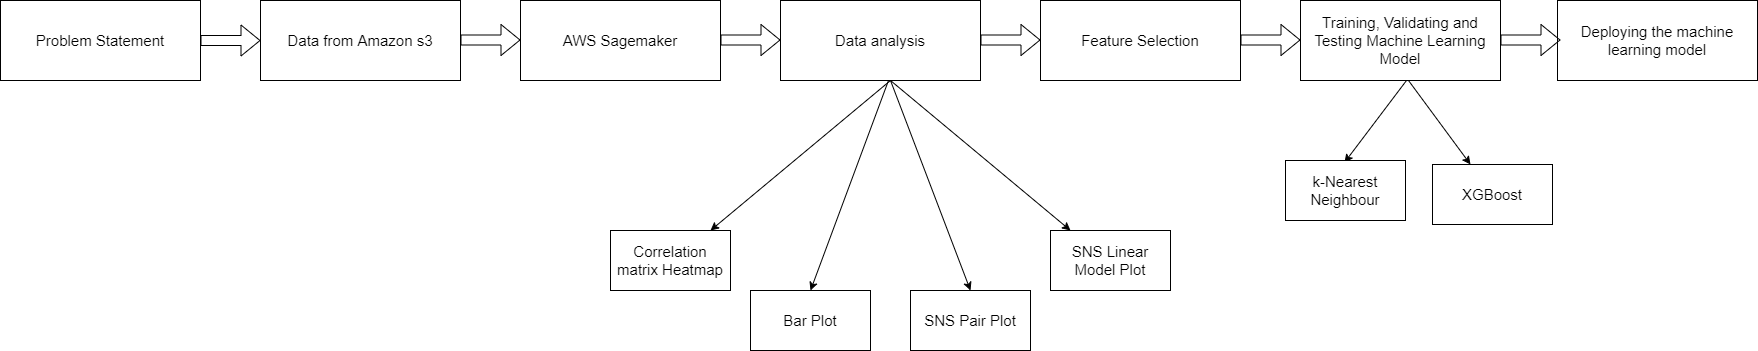
\includegraphics[width=1\linewidth]{pages/Chapter3/Chapter 3 images/Ml.PNG}
    \caption{Machine Learning Process Pipeline - \textit{Full scale diagram is in Appendix B} 
      [\ref{appendix:ML process pipeline}]}
    \label{Machine Learning Process Pipeline}
\end{figure}

The following steps to be carried out are as stated below:
\begin{itemize}
    \item Data stored as JSON files in buckets in the s3 cloud storage is imported into AWS Sagemaker with granted permission access. The code will be written in the Python programming language in JupyterLab. 
    \item Data is analysed using several methods such as correlation matrix, sns pair plots, bar plots and sns linear model plots to find correlation between parameters of the telemetry data.
    \item Useful parameters are extracted and used as features from the data analysis process. 
    \item Features selected are split into a 70:20:10 ratio for training, validating and testing the machine learning model respectively.
    \item Supervised learning algorithms such as XGBoost and k-Nearest Neighbour are used to train the ML model with hyperparameters tuned using the validating set. Testing set is used to evaluate the final performance of the machine learning model.
     \item The performance of the ML model will be evaluated with a confusion matrix with metrics such as accuracy.
    \item The ML model will be deployed after achieving a satisfying performance.
\end{itemize}

The trained machine learning model can be deployed for inference of real-time data. An endpoint will be created automatically once the model is deployed in Sagemaker. The endpoint created for the machine learning model can be invoked in the AWS cloud service.
Using Amazon API Gateway and AWS Lambda services, the endpoint can be invoked to allow the machine learning model to predict new data. To do this, a Lambda function that calls model is first created. An IAM execution role that includes a policy is chosen to give permission access to the Lambda function to invoke the model endpoint. An API gateway will then be created and deployed for the lambda function. This API will trigger an event that invokes the Lambda function where it passes data. Postman, an HTTP client for test service is used for the testing phase of the model endpoint. An invoked URL provided will be entered onto Postman with the data included in it. The prediction results on the data passed into Postman by the ML model will then be displayed on the interface. 


